
\chapter{Conceptual Model for Reactive Information Systems and their Services}
% \\...Reactive Web Systems
% \\...Reactive Services
% \\...Web-based Event-Action Services}
% NOTES / TODOs:
%
% Rahmenbedingungen
% Vorzuege
% Notwendigkeiten
% Architektur
% Schema: Zeit / Verteiltheit
%

% Steckbrief von Prototyp erstellen
 % was muss man ausfüllen um UC zu erstellen?

 % top down now, show whats beautiful and get everything together to get there

% NOTES / TODOs:
%

% why are we now suddenly responsive? we loosened up certain things

% TODO why JS. JSON as first advantage (http://www.toptal.com/nodejs/why-the-hell-would-i-use-node-js)
% advantage for network applications with several concurrent connections
% not as client-server used as intented but as serverserver com since we also expect several connections simultanously under load.
% But also, we adopt the non-blocking nature of JS that is used for node's optimal communication, in order to implement our enigne in a non blocking way, thus allowing to load code and fire callback function in modules whenever they are required!
% http://ariya.ofilabs.com/2012/07/lazy-parsing-in-javascript-engines.html
% Optimization of special case if ( before function {immediately-invoked function expression (IIFE)}, do rela parsing, else lazy parsing
% Difference between context and scope. scope unique to each invocation, context is 'this', owner of currently executing code.
% .call, .apply 
% TODO we should use .bind for persistence.coffee's functions ....

%In JavaScript, functions are first-class objects, i.e. they are objects and can be manipulated and passed around just like any other object. Specifically, they are Function objects. -> https://developer.mozilla.org/en/docs/Web/JavaScript/Reference/Functions_and_function_scope
% Since each call provides potentially different arguments, a new closure is created for each call to outside. The memory can be freed only when the returned inside is no longer accessible

% The definitive guide: This combination of a function object and a scope (a set of variable bindings) in which the function’s variables are resolved is called a closure in the computer science literature.4
% This is an old term that refers to the fact that the function’s variables have bindings in the scope chain and that therefore the function is “closed over” its variables.

\section{The Web as Request Handler}
% Classify Actions in information space

\section{The Web as Event Producer}
% Classify events in information space

\section{From Web Events to Web Actions}
% \subsection{Engine \& Rules}
% TODO conditions with examples
% Model / Schema
% Zeit / Verteiltheit

% RL <-> ECA
% TODO figure: ECA Schema
% TODO Figure: ECA in the distributed environemnt
% TODO figure: Rules (unions / objects / Rueckkoppelungen )

% \section{Event Condition Action (ECA) Model in the Web}
In the last section we showed how mashups create additional value for the web by combining several WebAPI's.
But it turned out, that such mashups are closed systems, which ofen only allow little degree of parametrization.
To get past such limitations and define a conceptual model for reactive web systems, it is necessary to define a 

existing rule languages, rule engines, 

Existing ECA systems all act on local data.
% (List examples) 
Looking at (Wikipedia...) their definition is actions on local data.
This does only add reactivity to these systems and not to the Web per se.

Such systems are merely event sinks which add fairly any value to the Web, except for the individual users and the system itself.

\begin{figure}[!ht]
  \centering
  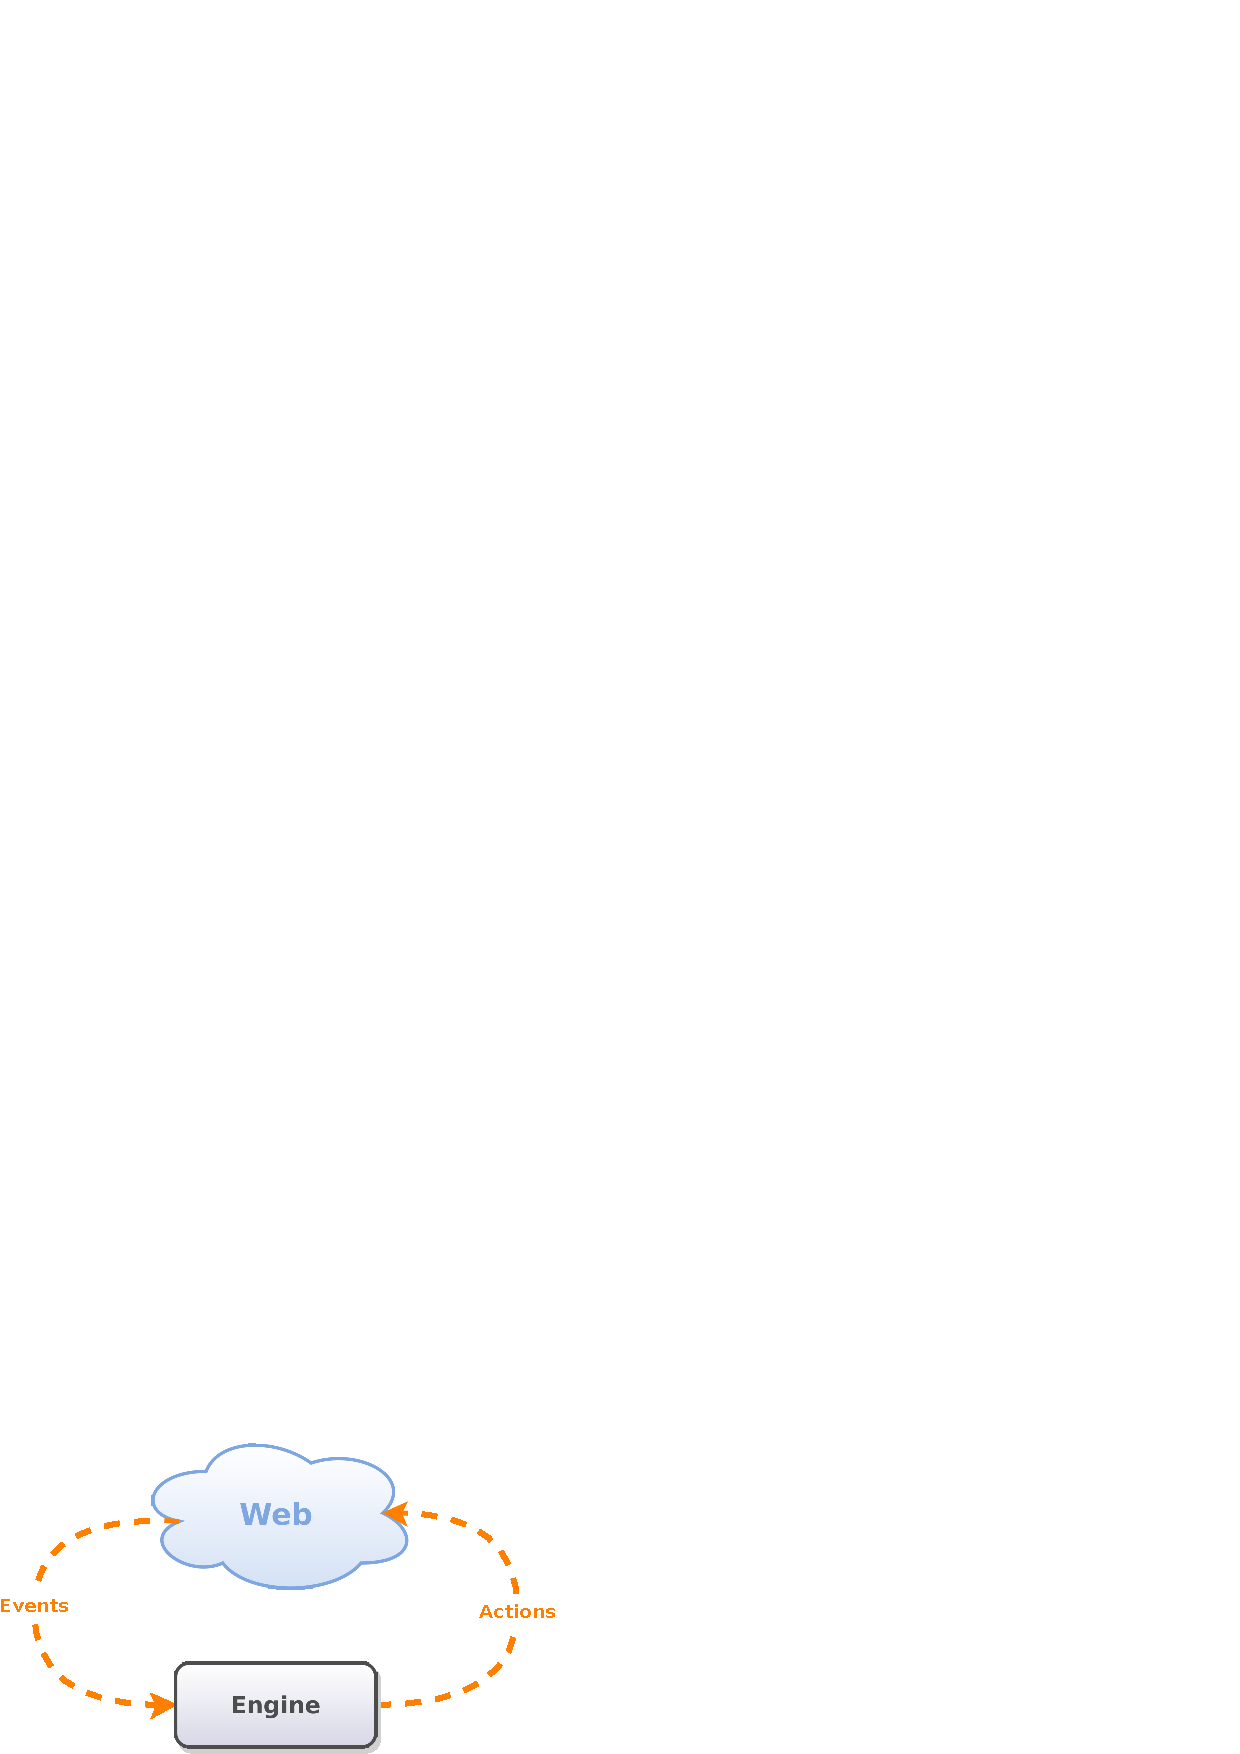
\includegraphics{figures/Conceptual_Model_Simple}
  \caption{Reactor ;) Conceptual model for reactive web systems}
  \label{fig:Conceptual_Model_Simple}
\end{figure}

\begin{figure}[!ht]
  \centering
  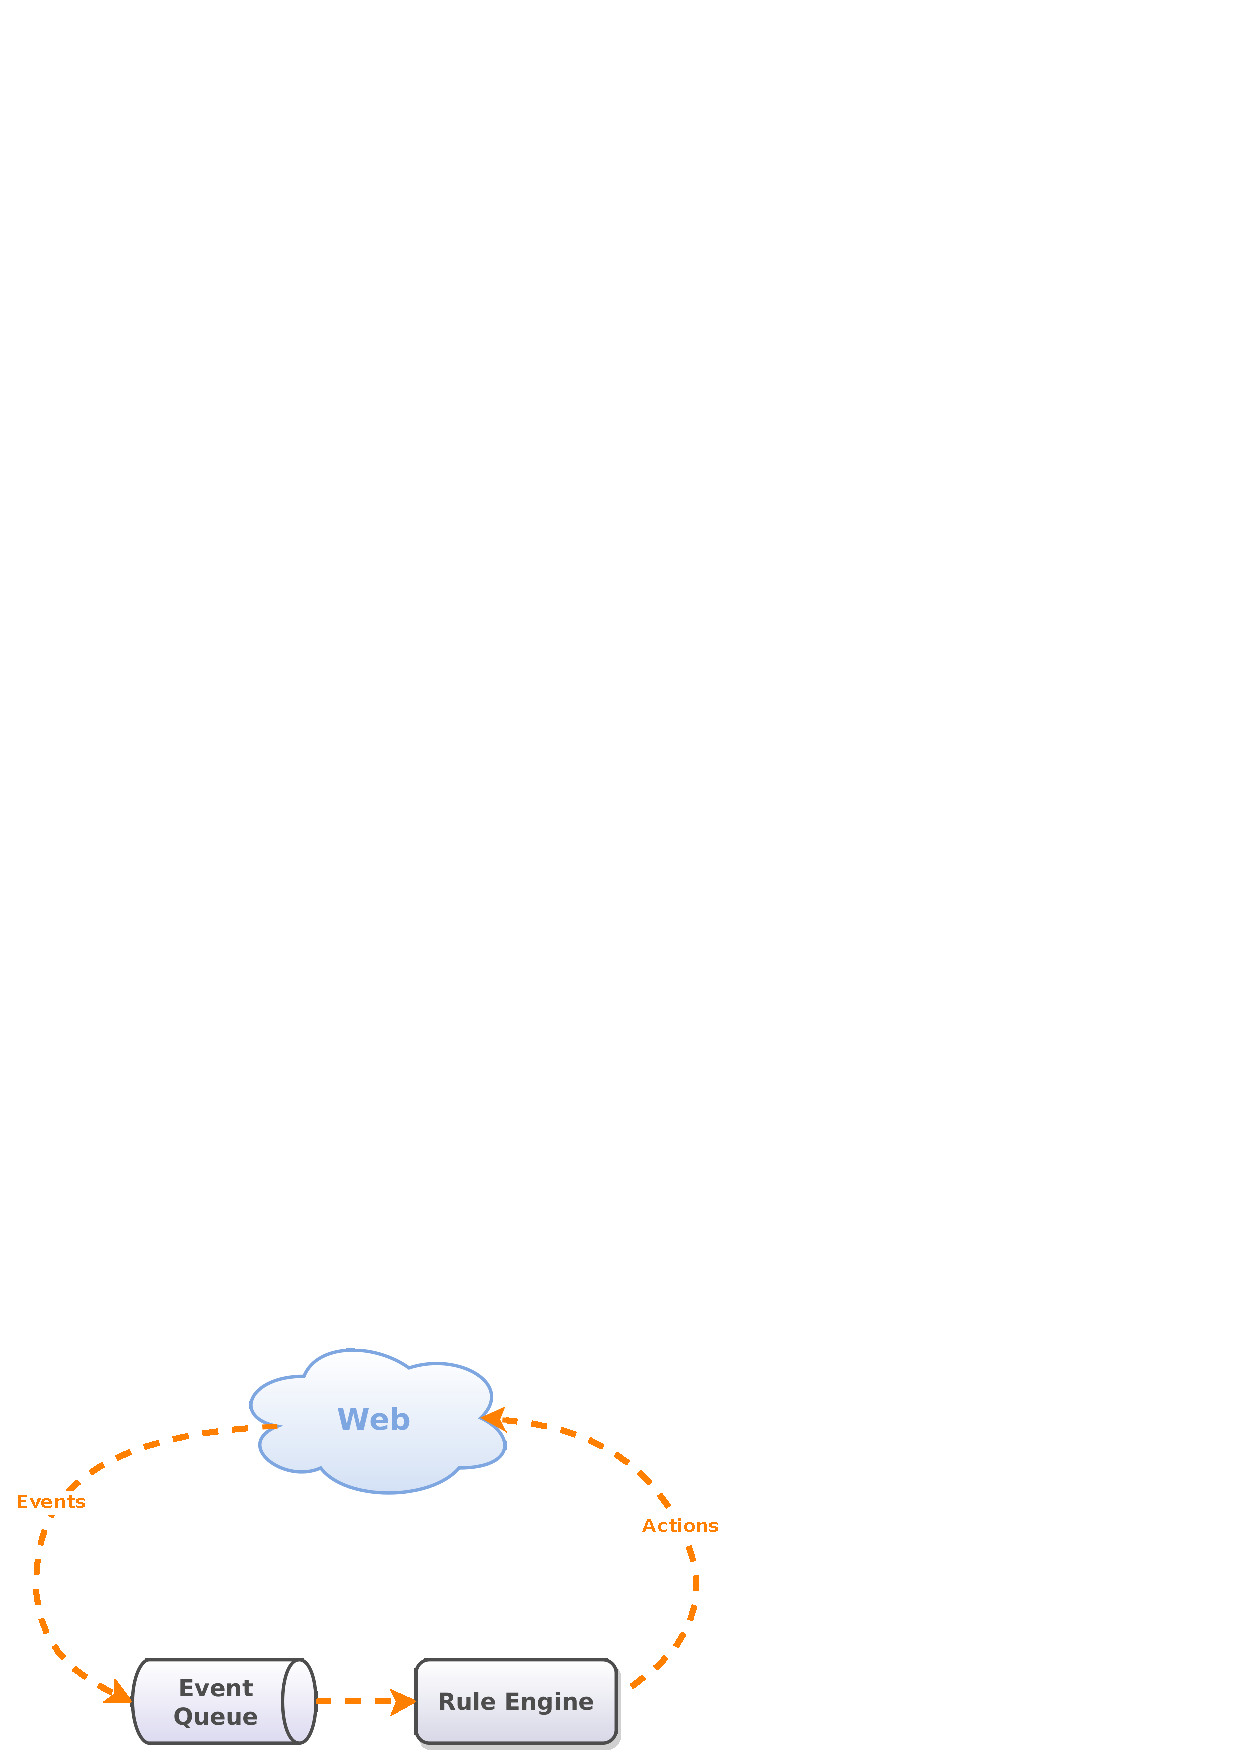
\includegraphics{figures/Conceptual_Model}
  \caption{Conceptual model for reactive Web Systems}
  \label{fig:Conceptual_Model}
\end{figure}


\begin{itemize}
  \item from web to events
  \item from events to rules
  \item from rules to actions
  \item from actions to the Web
  \item from concept to engine
\end{itemize}


% Regelimplementierungssprache
\subsection{Conceptual Rule Language}
Describe conceptual rule language
ON (existing categories)
IF (condition boundaries)
DO (call to existing action modules with parameters)

a lot possible, but dangerous.

\begin{Verbatim}[fontsize=\small,commandchars=\\\{\}]
\PY{k}{on} \PY{n}{mail}
\PY{k}{if} \PY{n}{sender}\PY{o}{=}\PY{l+s+ss}{\PYZdq{}sender@mail.com\PYZdq{}}
\PY{k}{do} \PY{n}{webapi}\PY{o}{\PYZhy{}}\PY{o}{\PYZgt{}}\PY{l+s+s2}{newcontent}\PY{p}{(}\PY{n}{subject}\PY{p}{)}
\end{Verbatim}
